% Appendix Template

\chapter{Results of experiment 2.1} % Main appendix title

\label{Appendix2-1} % Change X to a consecutive letter; for referencing this appendix elsewhere, use \ref{AppendixX}


\begin{figure}[ht]
  \centering
  \begin{subfigure}[b]{0.5\linewidth}
    \centering\captionsetup{width=.8\linewidth}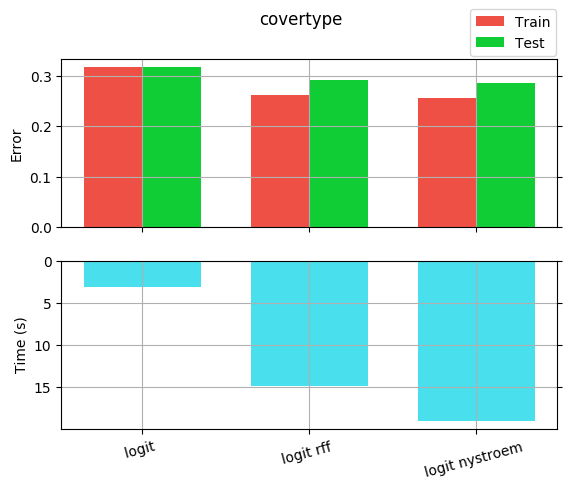
\includegraphics[width=\imgscale\linewidth]{Figures/2_1/covertype}
    \caption{prueba covertype}
    \label{fig:2_1_covertype}
  \end{subfigure}%
  \begin{subfigure}[b]{0.5\linewidth}
    \centering\captionsetup{width=.8\linewidth}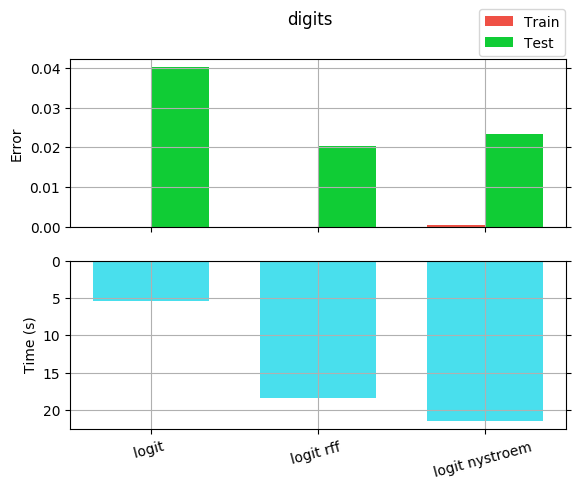
\includegraphics[width=\imgscale\linewidth]{Figures/2_1/digits}
    \caption{prueba digits}
    \label{fig:2_1_digits}
  \end{subfigure}
\end{figure}

\begin{figure}[ht]
  \centering
  \begin{subfigure}[b]{0.5\linewidth}
    \centering\captionsetup{width=.8\linewidth}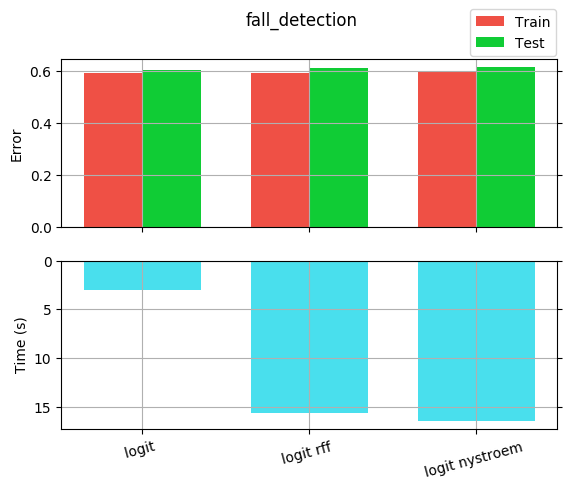
\includegraphics[width=\imgscale\linewidth]{Figures/2_1/fall_detection}
    \caption{prueba fall-detection}
    \label{fig:2_1_fall_detection}
  \end{subfigure}%
  \begin{subfigure}[b]{0.5\linewidth}
    \centering\captionsetup{width=.8\linewidth}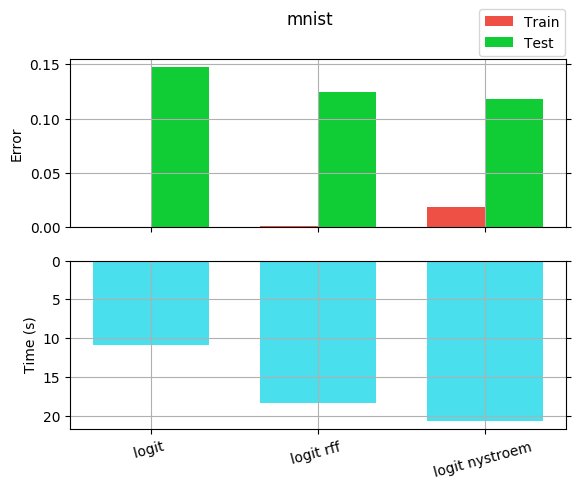
\includegraphics[width=\imgscale\linewidth]{Figures/2_1/mnist}
    \caption{prueba mnist}
    \label{fig:2_1_mnist}
  \end{subfigure}
\end{figure}


\begin{figure}[ht]
  \centering
  \begin{subfigure}[b]{0.5\linewidth}
    \centering\captionsetup{width=.8\linewidth}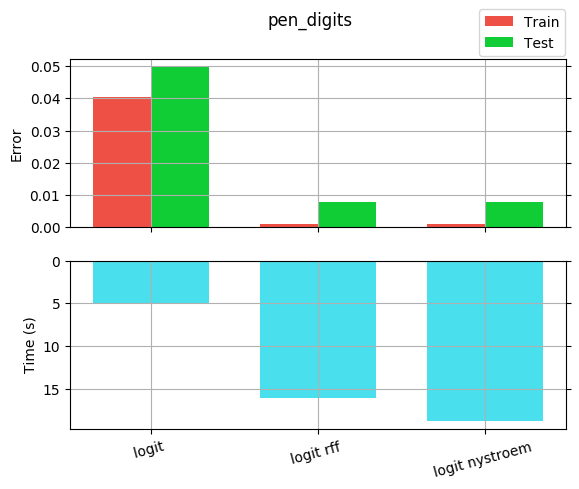
\includegraphics[width=\imgscale\linewidth]{Figures/2_1/pen_digits}
    \caption{prueba pen-digits}
    \label{fig:2_1_pen_digits}
  \end{subfigure}%
  \begin{subfigure}[b]{0.5\linewidth}
    \centering\captionsetup{width=.8\linewidth}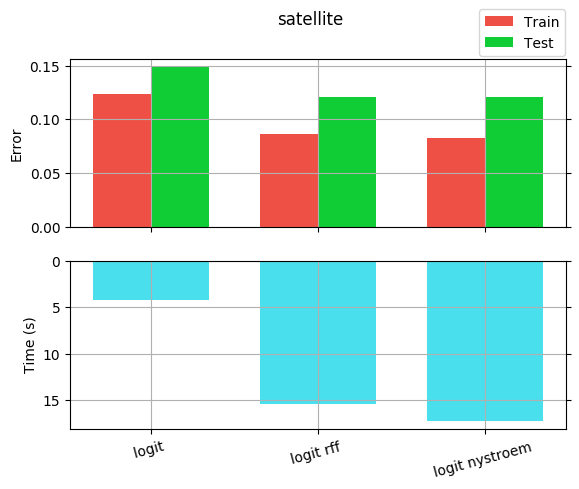
\includegraphics[width=\imgscale\linewidth]{Figures/2_1/satellite}
    \caption{prueba satellite}
    \label{fig:2_1_satellite}
  \end{subfigure}
\end{figure}

\begin{figure}[ht]
  \centering
  \begin{subfigure}[b]{0.5\linewidth}
    \centering\captionsetup{width=.8\linewidth}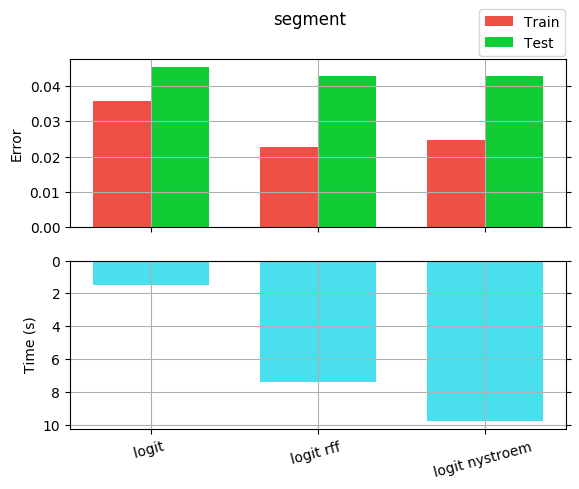
\includegraphics[width=\imgscale\linewidth]{Figures/2_1/segment}
    \caption{prueba segment}
    \label{fig:2_1_segment}
  \end{subfigure}%
  \begin{subfigure}[b]{0.5\linewidth}
    \centering\captionsetup{width=.8\linewidth}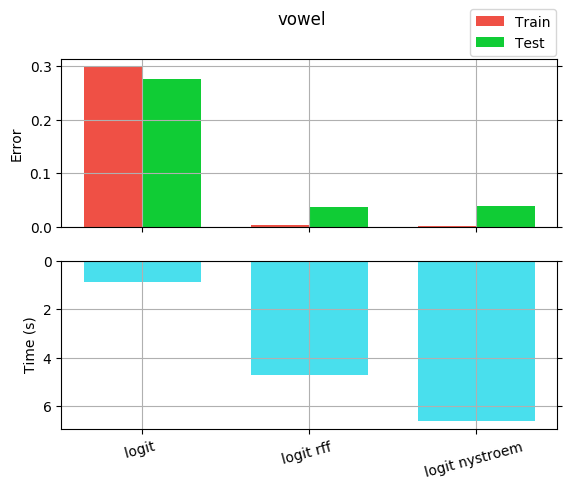
\includegraphics[width=\imgscale\linewidth]{Figures/2_1/vowel}
    \caption{prueba vowel}
    \label{fig:2_1_vowel}
  \end{subfigure}
\end{figure}
